% https://github.com/jgm/pandoc-templates/blob/master/default.latex
% http://rmarkdown.rstudio.com/pdf_document_format.html#custom_templates

\documentclass[12pt, oneside]{book}
\usepackage{lmodern}
\usepackage{amssymb,amsmath}
\usepackage{ifxetex,ifluatex}
\usepackage{fixltx2e} % provides \textsubscript
\ifnum 0\ifxetex 1\fi\ifluatex 1\fi=0 % if pdftex
  \usepackage[T1]{fontenc}
  \usepackage[utf8]{inputenc}
\else % if luatex or xelatex
  \usepackage{unicode-math}
  \defaultfontfeatures{Ligatures=TeX,Scale=MatchLowercase}
\fi
% use upquote if available, for straight quotes in verbatim environments
\IfFileExists{upquote.sty}{\usepackage{upquote}}{}
% use microtype if available
\IfFileExists{microtype.sty}{%
\usepackage[]{microtype}
\UseMicrotypeSet[protrusion]{basicmath} % disable protrusion for tt fonts
}{}
\PassOptionsToPackage{hyphens}{url} % url is loaded by hyperref
\usepackage[unicode=true]{hyperref}
\hypersetup{
            pdftitle={A Study in Disaster},
            pdfauthor={mauveSushi},
            pdfborder={0 0 0},
            breaklinks=true}
\urlstyle{same}  % don't use monospace font for urls





%%%%%%%%%%%%%%%%%%%%%%%%%%%%%%%%%%%%%%%%%%%%%%%%%%%%%
% CUSTOM
%%%%%%%%%%%%%%%%%%%%%%%%%%%%%%%%%%%%%%%%%%%%%%%%%%%%%

% margin
\usepackage[letterpaper, margin=1in]{geometry}
\usepackage{titlesec}
% change "Chapter" prefix in a book to "Section"

% hide chapter text
\renewcommand{\chaptername}{Section}
\titleformat{\chapter}{\normalfont\huge\bf}{\thechapter.}{20pt}{\huge\bf}

% title page style
\newcommand*{\titleGM}{\begingroup % Create the command for including the title page in the document
\hbox{ % Horizontal box
\hspace*{0.2\textwidth} % Whitespace to the left of the title page
\rule{1pt}{\textheight} % Vertical line
\hspace*{0.05\textwidth} % Whitespace between the vertical line and title page text
\parbox[b]{0.75\textwidth}{ % Paragraph box which restricts text to less than the width of the page
  {\noindent\Huge\bfseries A Study in Disaster}\\[2\baselineskip] % Title
  {\large \textit{The Titanic Survivors}}\\[4\baselineskip] % Tagline or further description
  {\Large \textsc{mauveSushi}} % Author name

  \vspace{0.5\textheight} % Whitespace between the title block and the publisher
  {\noindent\large Skidmore College}\\[\baselineskip] % Publisher and logo
  }
}
\endgroup}

%%%%%%%%%%%%%%%%%%%%%%%%%%%%%%%%%%%%%%%%%%%%%%%%%%%%%






\usepackage{natbib}
\bibliographystyle{apalike}
\usepackage{longtable,booktabs}
% Fix footnotes in tables (requires footnote package)
\IfFileExists{footnote.sty}{\usepackage{footnote}\makesavenoteenv{long table}}{}
\usepackage{graphicx,grffile}
\makeatletter
\def\maxwidth{\ifdim\Gin@nat@width>\linewidth\linewidth\else\Gin@nat@width\fi}
\def\maxheight{\ifdim\Gin@nat@height>\textheight\textheight\else\Gin@nat@height\fi}
\makeatother
% Scale images if necessary, so that they will not overflow the page
% margins by default, and it is still possible to overwrite the defaults
% using explicit options in \includegraphics[width, height, ...]{}
\setkeys{Gin}{width=\maxwidth,height=\maxheight,keepaspectratio}
\IfFileExists{parskip.sty}{%
\usepackage{parskip}
}{% else
\setlength{\parindent}{0pt}
\setlength{\parskip}{6pt plus 2pt minus 1pt}
}
\setlength{\emergencystretch}{3em}  % prevent overfull lines
\providecommand{\tightlist}{%
  \setlength{\itemsep}{0pt}\setlength{\parskip}{0pt}}
\setcounter{secnumdepth}{5}
% Redefines (sub)paragraphs to behave more like sections
\ifx\paragraph\undefined\else
\let\oldparagraph\paragraph
\renewcommand{\paragraph}[1]{\oldparagraph{#1}\mbox{}}
\fi
\ifx\subparagraph\undefined\else
\let\oldsubparagraph\subparagraph
\renewcommand{\subparagraph}[1]{\oldsubparagraph{#1}\mbox{}}
\fi

% set default figure placement to htbp
\makeatletter
\def\fps@figure{htbp}
\makeatother

\usepackage{booktabs}
\usepackage{longtable}
\usepackage{hyperref}
\usepackage{amsthm}
\usepackage[dvipsnames,table,xcdraw]{xcolor}
\usepackage[breakable, theorems, skins]{tcolorbox}

% color palette
\definecolor{Azure}{rgb}{0.0, 0.5, 1.0}

\makeatletter
% adjust theorem spacing
\def\thm@space@setup{%
  \thm@preskip=8pt plus 2pt minus 4pt
  \thm@postskip=\thm@preskip
}

% colorie hyperlink
\hypersetup{
    colorlinks=true,
    citecolor={black},
    linkcolor={black},
    menucolor={black},
    urlcolor={Azure}
}

% make function greybox
\DeclareRobustCommand{\greybox}[2][gray!10]{%
\begin{tcolorbox}[   %% Adjust the following parameters at will.
        breakable,
        left=0pt,
        right=0pt,
        top=0pt,
        bottom=0pt,
        colback=#1,
        colframe=#1,
        width=\dimexpr\textwidth\relax, 
        enlarge left by=0mm,
        boxsep=5pt,
        arc=0pt,outer arc=0pt,
        ]
        #2
\end{tcolorbox}
}

\makeatother

\title{A Study in Disaster}
\author{mauveSushi}
\date{2017-12-13}



%%%%%%%%%%%%%%%%%%%%%%%%%%%%%%%%%%%%%%%%%%%%%%%%%%%%%
% DOCUMENT BEGIN
%%%%%%%%%%%%%%%%%%%%%%%%%%%%%%%%%%%%%%%%%%%%%%%%%%%%%

\usepackage{amsthm}
\newtheorem{theorem}{Theorem}[chapter]
\newtheorem{lemma}{Lemma}[chapter]
\theoremstyle{definition}
\newtheorem{definition}{Definition}[chapter]
\newtheorem{corollary}{Corollary}[chapter]
\newtheorem{proposition}{Proposition}[chapter]
\theoremstyle{definition}
\newtheorem{example}{Example}[chapter]
\theoremstyle{definition}
\newtheorem{exercise}{Exercise}[chapter]
\theoremstyle{remark}
\newtheorem*{remark}{Remark}
\newtheorem*{solution}{Solution}
\begin{document}
% replace the default title page by removing \maketitle
% % \maketitle
% 
\pagestyle{empty}  % Removes page numbers need the blank line before of this line
\titleGM


\fontsize{12}{16}\selectfont

\hypertarget{abstract}{%
\chapter*{Abstract}\label{abstract}}
\addcontentsline{toc}{chapter}{Abstract}

This research aims to construct a logistic regression model to predict
the survival outcome of passenger on the Titanic based on their various
demographic and socioeconomic factors, such as age, gender, number of
spouses and siblings, passenger class, etc. The findings of this
research can be generalized to most shipwreck where the ship is
considered big (having capacity of at least 1000 passengers) and the
route is through Atlantic Ocean in the early 20\textsuperscript{th}
century. We used logistic regression in tandem with backward feature
selection to obtain several prediction models. We evaluate each obtained
model using the Hosmer-Lemeshow goodness-of-fit test and then conduct a
more vigorous feature selection process to come up with the best models.
Despite the different approaches, all of the obtained models suggest a
common trend that children, female and first class passengers are among
the ones with highest chance of survival.

\hypertarget{introduction}{%
\chapter*{Introduction}\label{introduction}}
\addcontentsline{toc}{chapter}{Introduction}

On that fateful night April 15, 1912, the great Titanic carrying 2,200
people struck an iceberg and sank, brought down with it 1,500 poor
souls. Such tragedy never fails to leave all of us unsettled, but as
statisticians, we are naturally drawn to ask ourselves the question:
\emph{``How do demographic and socioeconomic factors affect chance of
survival in disaster?''} Perhaps, based on just the titanic data set,
such general question cannot be answered, since our findings are
probably just generelizable to a specific type of disaster, which is
shipwreck and to a time-frame limited to the early
20\textsuperscript{th} century. Also, we have to consider the fact that
Titanic is not just another ship\ldots{} It is (even till today) one of
the most luxurious ship ever been built (see figure below - the ship
even had swimming pool and tennis court at the lowest level!). As such,
we think the findings we obtain using this data set can only be
generalized to big ships, i.e.~ships whose capacity is at least 1000,
crossing the Atlantic ocean. Note that this number 1000 seems rather
arbitrary, but we found that nowadays, on average, cruise ships with
tonnage of around 40,000 usually have capacity of 1,000
passengers\footnote{CruiserMapper,
  \href{http://www.cruisemapper.com/wiki/761-cruise-ship-passenger-capacity-ratings}{Cruise
  Ship Passenger Capacity}} and most of the bigger ships in early
20\textsuperscript{th} century were around 40,000 or more in
tonnage\footnote{Wikipedia,
  \href{https://en.wikipedia.org/wiki/List_of_largest_passenger_ships}{List
  of largest passenger ships}}. For this reason, we formulate our
research question as follows:

\textbf{``How do various demographic and socioeconomic factors affect
chance of survival in shipwreck where the ship's capacity is at least
1000 passegners and the route is through the Atlantic Ocean in the early
20\textsuperscript{th} century?''}

In simpler words, we will attempt to create a model to be able to
predict the survival outcome of a passenger, given his/her relevant
background information. We constructed several different models with 2
major approaches, one using backward selection and one using a more
rigorous feature selection process. Despite this, the models we obtain
show a common trend that female, little kids and first-class passengers
are more likely to survive the shipwreck. Following this, we will step
by step present our data preparation and modelling process, as well as
our findings.

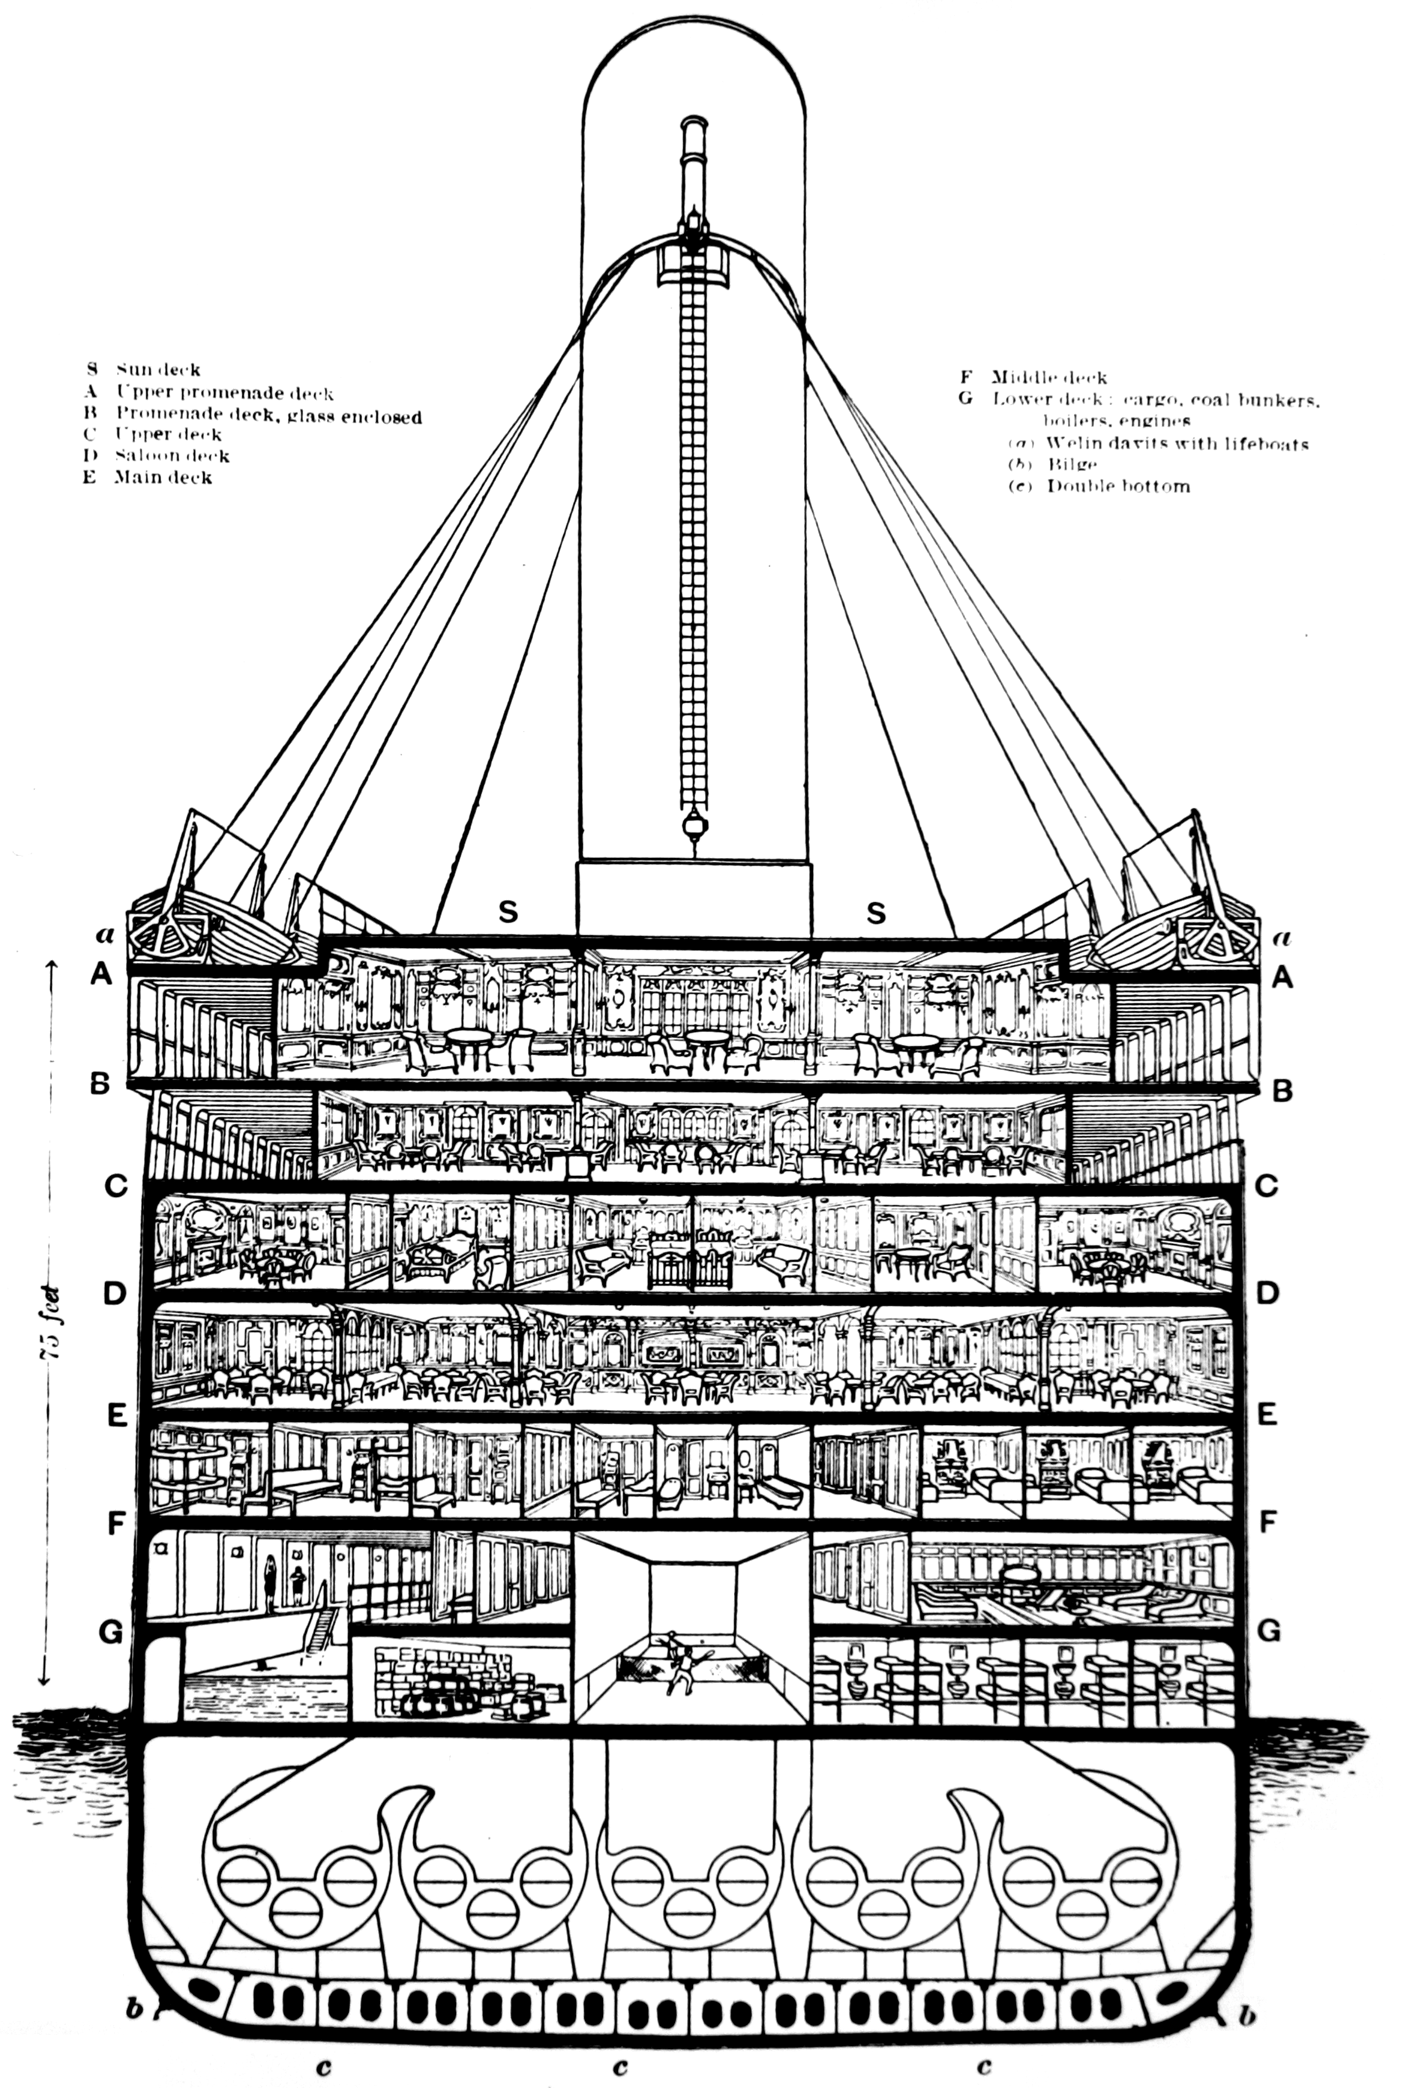
\includegraphics{assets/cross_section.png}

\hypertarget{data_explore}{%
\chapter{Data Exploration}\label{data_explore}}

\hypertarget{summary}{%
\section{Summary}\label{summary}}

The data set contains information about 1306 passengers on the Titanic.
Recall that there were around 2,200 people on the ship so with this
sample size, clearly the data set is a good representation of the
population on the Titanic. There are 11 variables in the original data
set, listed as follows:

\begin{tabular}{llllll}
\toprule
Name & Type & Unit & Meaning & Value/Range & Remark\\
\midrule
survival & nominal &  & previous name of county & 0 = No, 1 = Yes & \\
name & nominal &  & passenger's name &  & \\
pclass & ordinal &  & ticket class & 1 = 1st, 2 = 2nd, 3 = 3rd & We can use this as a proxy for socio-economic status (SES)\\
sex & nominal &  & passenger's gender & m = male, f = female & \\
age & numerical & year & passenger's age & [0,80] & \\
\addlinespace
sibsp & numerical & person & number of siblings/spouses aboard the Titanic & [0,8] & siblings = brother, sister, stepbrother, stepsister; spouses = husband, wife (mistresses and fiances were ignored)\\
parch & numerical & person & number of parents/children aboard the Titanic & [0,6] & parents = mother, father; children = son, daughter, stepson and stepdaughter (some children travelled only with nanny, therefore parch = 0 for them)\\
ticket & nominal &  & ticket number &  & \\
fare & numerical & pound & ticket fare & [0, 93.5] & \\
cabin & nominal &  & cabin number &  & \\
embarked & nominal &  & port of embarkation & C = Cherbourg, Q = Queenstown, S = Southampton & \\
\bottomrule
\end{tabular}

\hypertarget{variable-selection}{%
\section{Variable Selection}\label{variable-selection}}

Our response variable is the nominal variable \texttt{survival} (or
boolean as its outcome is 0 or 1). As for explanatory variables, we have
to make some pre-selection beforehand. We decide to take out several
variables which we consider only as identifier variables, such as
\texttt{name} and \texttt{ticket} number. Also we did not include the
\texttt{cabin} number since this information is missing for too many
passengers. The only value it brings to the model is when we can
actually compute the shortest distance from each cabin to the rescue
area. However, again as mentioned, there are a lot of missing data and
also, if distance is our only concern, then passenger class is quite
sufficient for this purpose (refer to the cross-section plot of the
Titanic in previous section).

\hypertarget{data-preparation}{%
\section{Data Preparation}\label{data-preparation}}

We notice that \texttt{age} is missing for many passenger, but
\texttt{age} is such a crucial variable that we cannot simply take away.
As such, we discretize age into several bins: missing, 0-5, 6-18, 19-55,
and 56 and above. Also, we rename the variables for readability. So the
final model we obtained has the following variables:

\begin{tabular}{llll}
\toprule
Name & Type & Unit & Value/Range\\
\midrule
has\_survived & nominal &  & 0 = No, 1 = Yes\\
passenger\_class & ordinal &  & 1 = 1st, 2 = 2nd, 3 = 3rd\\
gender & nominal &  & male, female\\
age & nominal & year & [0,5], [6,18], [19,55], [56 and above], missing\\
number\_of\_siblings\_and\_spouses & numerical & person & [0,8]\\
\addlinespace
number\_of\_parents\_and\_children & numerical & person & [0,6]\\
fare & numerical & pound & [0, 93.5]\\
embarked\_from & nominal &  & C = Cherbourg, Q = Queenstown, S = Southampton\\
\bottomrule
\end{tabular}

\hypertarget{final-data-set-summary}{%
\section{Final Data Set Summary}\label{final-data-set-summary}}

Following is the summary of the final data set:

\begin{verbatim}
## has_survived
##   0   1 
## 808 498
\end{verbatim}

\begin{verbatim}
## gender
## female   male 
##    464    842
\end{verbatim}

\begin{verbatim}
## age
##       [0,5]     [19,55] [56, above)      [6,18]     missing 
##          56         790          57         140         263
\end{verbatim}

\begin{verbatim}
##  number_of_siblings_and_spouses number_of_parents_and_children
##  Min.   :0.0                    Min.   :0.0000                
##  1st Qu.:0.0                    1st Qu.:0.0000                
##  Median :0.0                    Median :0.0000                
##  Mean   :0.5                    Mean   :0.3859                
##  3rd Qu.:1.0                    3rd Qu.:0.0000                
##  Max.   :8.0                    Max.   :9.0000                
##       fare       
##  Min.   :  0.00  
##  1st Qu.:  7.90  
##  Median : 14.45  
##  Mean   : 33.22  
##  3rd Qu.: 31.27  
##  Max.   :512.33
\end{verbatim}

\begin{verbatim}
## passenger_class
##  first second  third 
##    321    277    708
\end{verbatim}

\begin{verbatim}
## embarked_from
##   C   Q   S 
## 270 123 913
\end{verbatim}

\hypertarget{correlation-investigation}{%
\section{Correlation Investigation}\label{correlation-investigation}}

Following, we create a plot matrix to investigate potential collinearity
between variables in our data set.

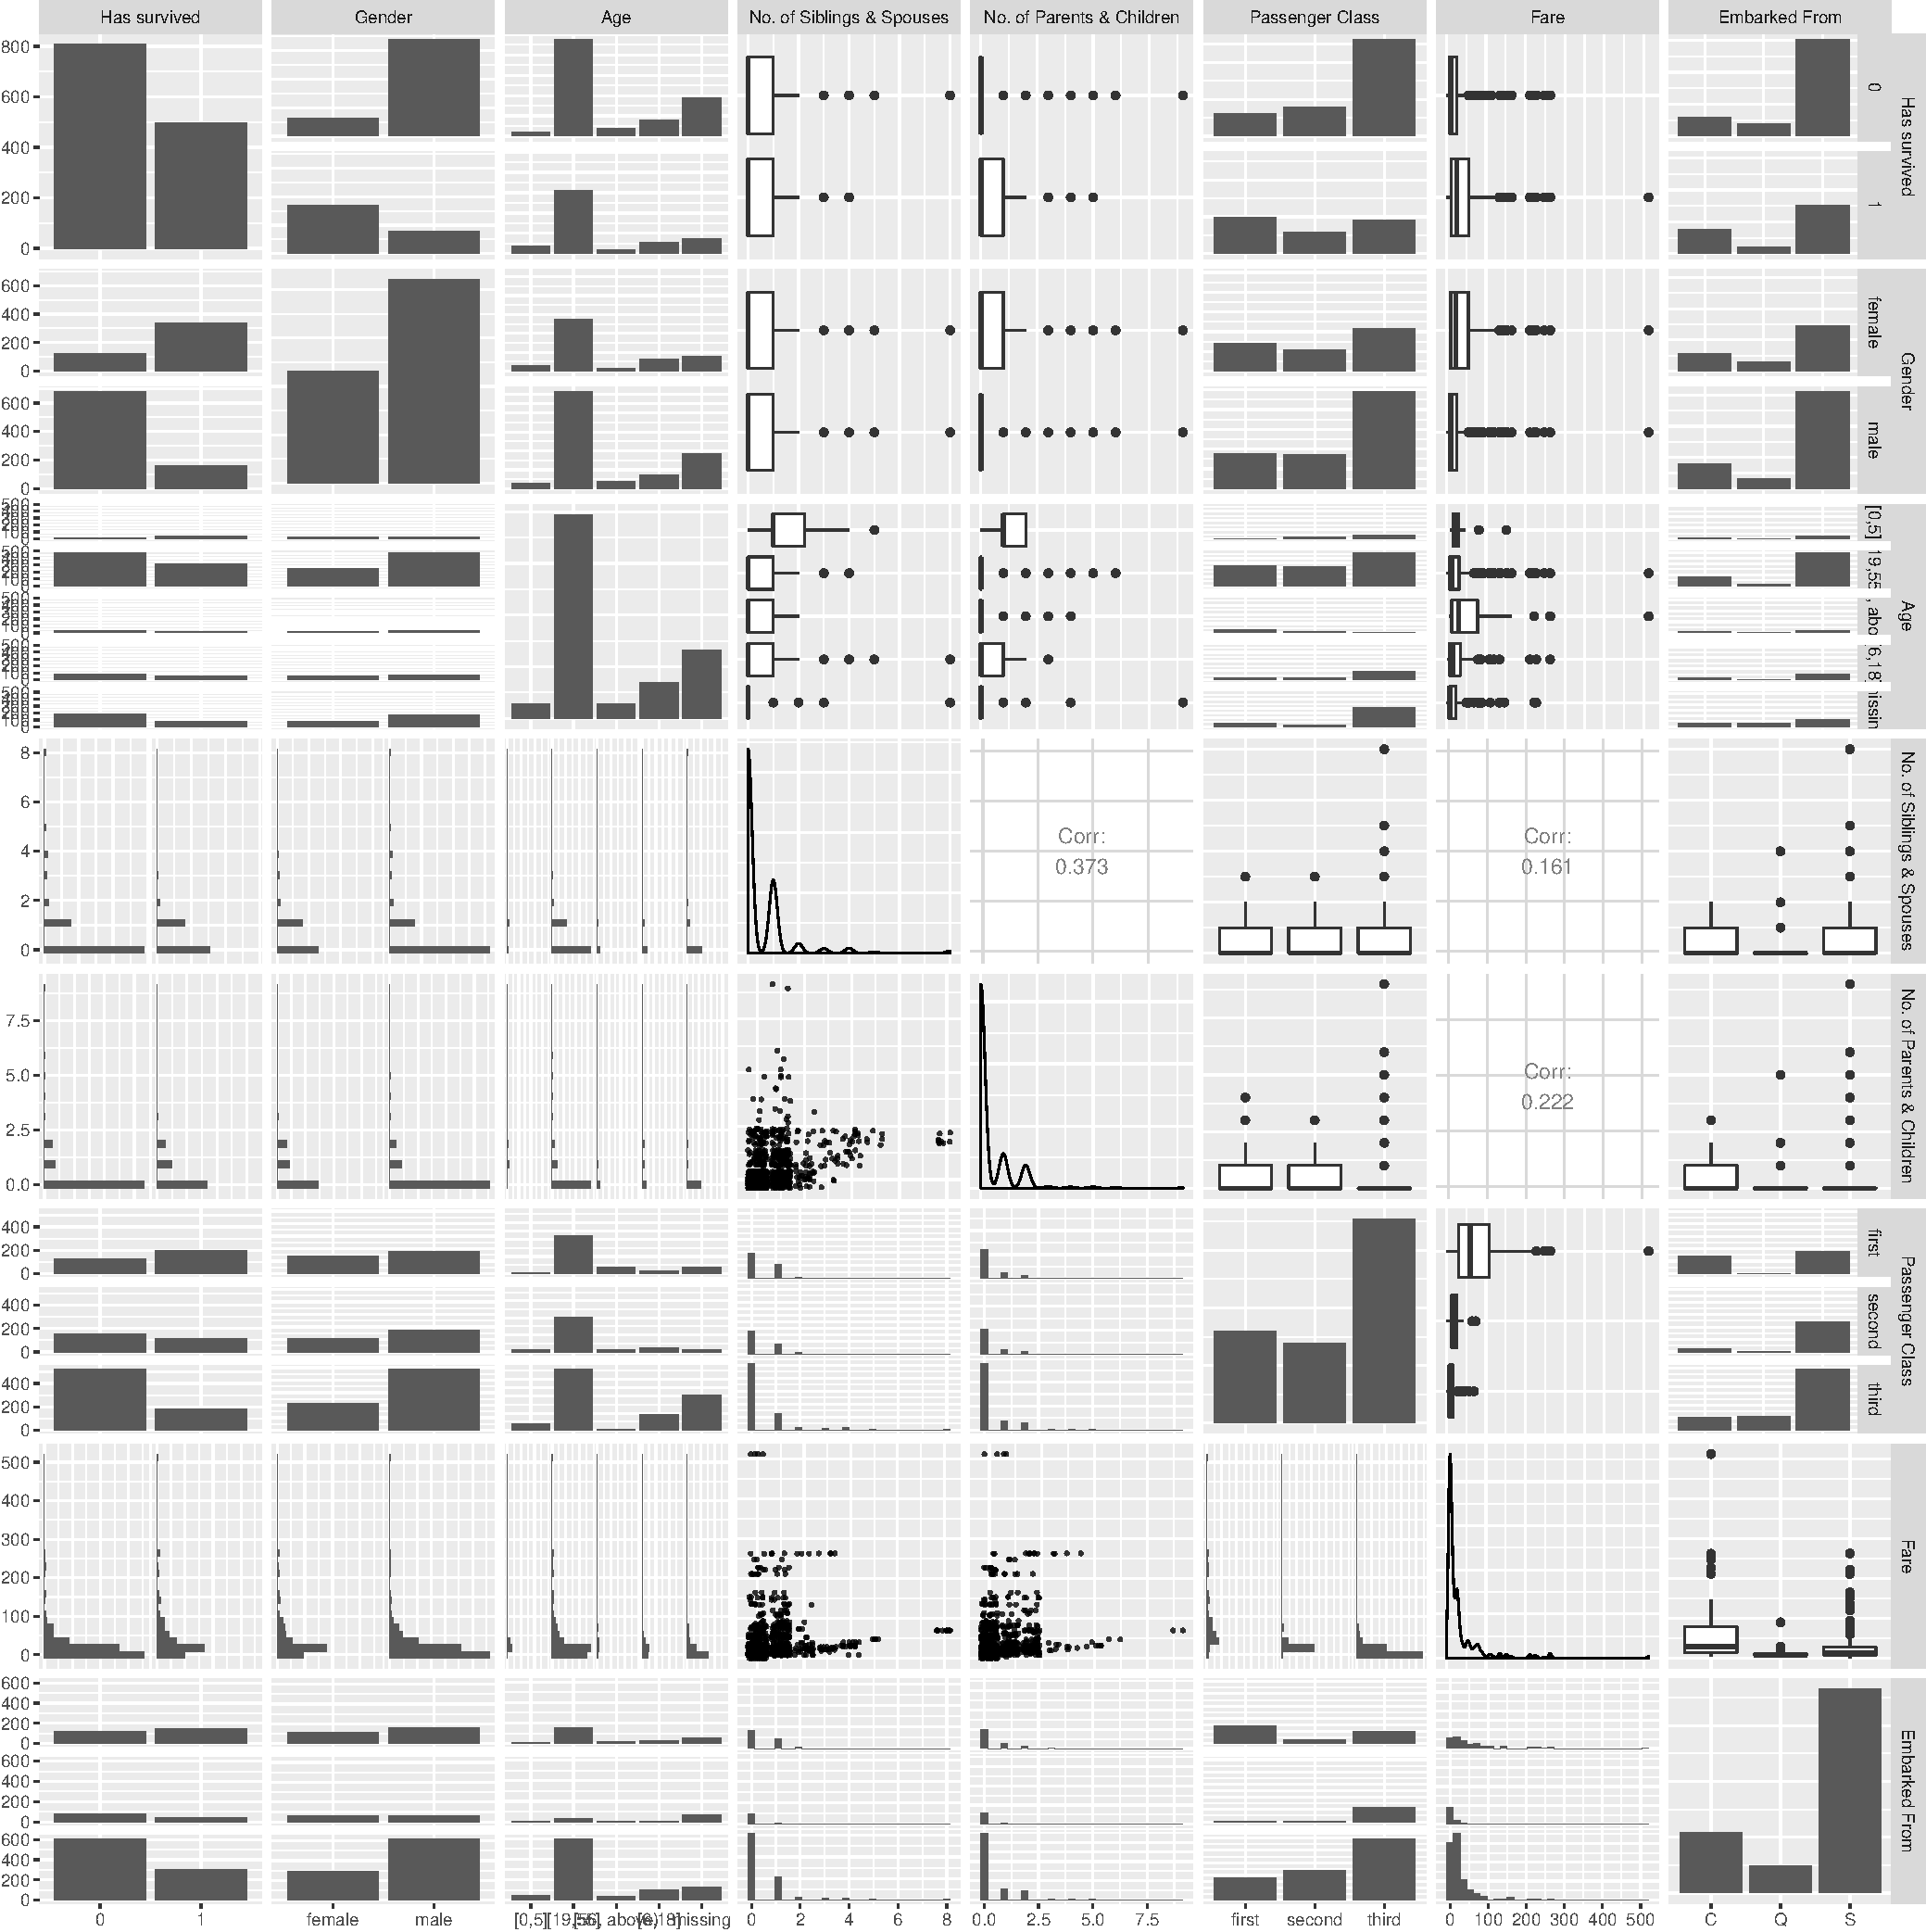
\includegraphics{report_files/figure-latex/unnamed-chunk-6-1.pdf}

As seen above, it seems that there might be some collinearity between
\texttt{gender} and \texttt{passenger\_class} as female and male groups
have very different first class to third class ratio. Also, notice that
\texttt{passenger\_class} and \texttt{embarked\_from} seem to have some
strong association, for example, there seems to be more third class
passenger embarking from Southampton than that of other embarkation
ports. As for now, we will take note of these observations; we will use
them later for a more vigorous feature selection process as we attempt
to improve our model.

\hypertarget{method}{%
\chapter{Methodology}\label{method}}

\hypertarget{backward-selection}{%
\section{Backward Selection}\label{backward-selection}}

For backward selection, we start out by including all of the variables
we have as explanatory variables and construct a regression model from
that. We then take out one of the insignificant predictor (predictor
whose p-value is greater than the significance level of 0.05 and whose
p-value is the greatest among all variables), and then construct another
model using the remaining variables. Repeat the process until we obtain
a model with all significant predictors.

\hypertarget{logistic-regression}{%
\section{Logistic Regression}\label{logistic-regression}}

In our project, since our response variable is a binary variable, we are
going to use logistic regression for the model. Logistic regression is a
type of generalized linear model. Its equation is in the form of
\(ln(\frac{p}{1-p})=\ln(odds)=\alpha_0+\alpha_1x_1+\alpha_2x_2+\dots +\alpha_nx_n\),
where \(p\), in this context, is the probability of survival--1 means
the passenger survived and 0 otherwise, and \(x_1, x_2, \dots, x_n\) are
explanatory variables. The right hand side of this equation is the same
as in a linear model, hence it is called generalized linear model. The
left-hand side is the natural log of odds, where odds is a
representation of probability, and it equals to \(\frac{p}{1-p}\). Once
we fit a model, we can predict the probability of success \(p\) by
\(p = \frac{1}{1+e^{-RHS}}\), where
\(RHS=\alpha_0+\alpha_1x_1+\alpha_2x_2+\dots +\alpha_nx_n\).

To perform logistic regression, we can use \texttt{glm()} function,
which stands for generalized linear model, in R, and specify the
parameter \texttt{family\ =\ binomial(link\ =\ "logit")}.

\hypertarget{homser-lemeshow-goodness-of-fit-test}{%
\section{Homser-Lemeshow Goodness-Of-Fit
Test}\label{homser-lemeshow-goodness-of-fit-test}}

Since we decided to use logistic regression for our model, the
assumptions we need to verify are not the same as in a linear regression
model. For example, we cannot plot a residual plot to see whether the
residuals have a pattern because however good or bad a model is, the
residuals will always show a pattern, as they follow 2 curves: positive
residuals follow the curve \(1 - \frac{1}{1+e^{-predicted}}\) and the
negative residuals follow the curve \(0 - \frac{1}{1+e^{-predicted}}\)
as seen below:

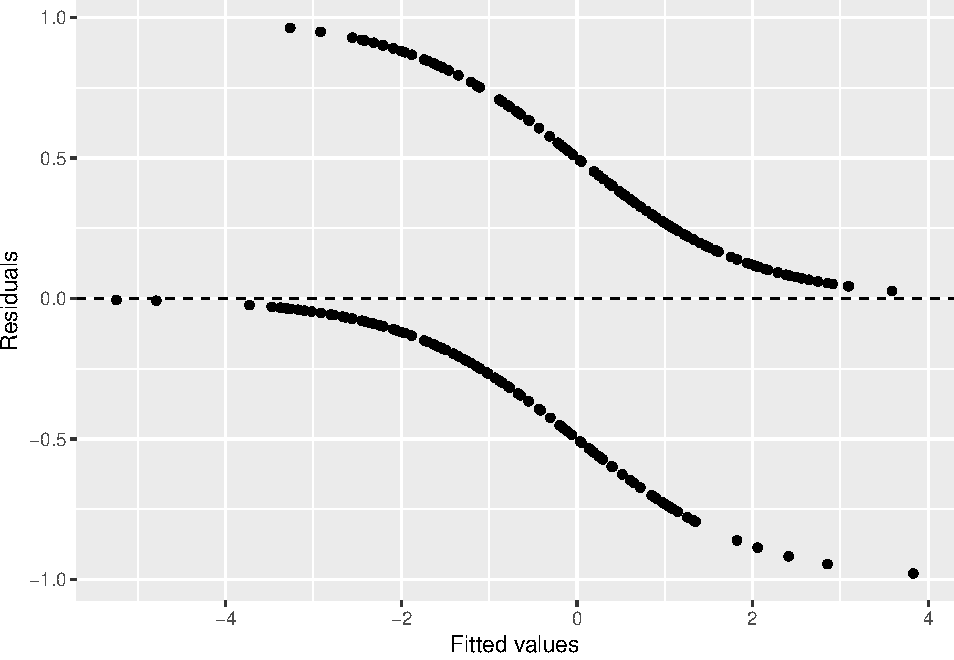
\includegraphics{report_files/figure-latex/unnamed-chunk-9-1.pdf}

To examine how good a logistic regression model is, we can use
Homser-Lemeshow goodness-of-fit test. The idea of this test is to divide
the sample into several groups according to their predicted values, and
compare the expected proportion of success to the observed proportion of
success in each group to see whether there is a significant difference
between the expected and the observed proportion. The null hypothesis of
this test is that there is no difference between the expected and the
observed proportion of success. In other words, if the p-value of this
test is too low, it means that we have strong evidence that the fit is
not good enough.

However, there are some restrictions for this test as well. One of which
is that the choice of number of groups may affect the p-value
significantly, and there is no clear rule for how to choose the most
proper number of groups. Also, it does not take overfitting into
consideration. Because of these problems, we will only use
Homser-Lemeshow goodness-of-fit test to give us a rough sense of how
good a model is, but not necessarily to reject that model altogether.

To perform Homser-Lemeshow goodness-of-fit test, we can use
\texttt{hoslem.test()} function in \texttt{ResourceSelection} package in
R.

\hypertarget{akaike-information-criterion-aic}{%
\section{Akaike Information Criterion
(AIC)}\label{akaike-information-criterion-aic}}

We will also use Akaike information criterion to evaluate our model.
This criterion is a method to compare several regression models
together. It is a function of the goodness-of-fit of a model and the
number of parameters it takes. It gives reward to better goodness-of-fit
and gives penalty to increasing number of explanatory variables The
advantage of this criterion is that it will give penalty to
over-fitting. However, the limitation of this method is that there is no
natural scale to compare with, so it is possible that all of our models
have poor fit, and we just choose the relatively best one among these.
In general, the lower the AIC value, the better the model is.

This is very convenient in R. It is included in the \texttt{summary()}
function and we can also call it using \texttt{AIC()} function.

\hypertarget{model}{%
\chapter{Model}\label{model}}

\hypertarget{model-obtained-using-backward-selection}{%
\section{Model Obtained Using Backward
Selection}\label{model-obtained-using-backward-selection}}

The first model we obtained is by backward selection. We eliminated
\texttt{number\_of\_siblings\_and\_spouses} and \texttt{fares} before we
obtained a model whose p-value of each variable is smaller than 0.05.
The model we obtained and its summary are shown below:

\begin{verbatim}
## 
## Call:
## glm(formula = has_survived ~ gender + age + number_of_siblings_and_spouses + 
##     passenger_class + embarked_from, family = binomial(link = "logit"), 
##     data = titanic)
## 
## Deviance Residuals: 
##     Min       1Q   Median       3Q      Max  
## -2.7755  -0.6791  -0.4560   0.7074   2.5697  
## 
## Coefficients:
##                                Estimate Std. Error z value Pr(>|z|)    
## (Intercept)                     4.86097    0.47163  10.307  < 2e-16 ***
## gendermale                     -2.60736    0.15798 -16.505  < 2e-16 ***
## age[19,55]                     -2.00712    0.38995  -5.147 2.65e-07 ***
## age[56, above)                 -3.10763    0.53229  -5.838 5.27e-09 ***
## age[6,18]                      -1.76429    0.43159  -4.088 4.35e-05 ***
## agemissing                     -2.21886    0.42028  -5.280 1.30e-07 ***
## number_of_siblings_and_spouses -0.35361    0.09297  -3.803 0.000143 ***
## passenger_classsecond          -0.91904    0.21489  -4.277 1.90e-05 ***
## passenger_classthird           -1.77251    0.19438  -9.119  < 2e-16 ***
## embarked_fromQ                 -0.47350    0.30504  -1.552 0.120601    
## embarked_fromS                 -0.67719    0.18791  -3.604 0.000314 ***
## ---
## Signif. codes:  0 '***' 0.001 '**' 0.01 '*' 0.05 '.' 0.1 ' ' 1
## 
## (Dispersion parameter for binomial family taken to be 1)
## 
##     Null deviance: 1736.2  on 1305  degrees of freedom
## Residual deviance: 1191.1  on 1295  degrees of freedom
## AIC: 1213.1
## 
## Number of Fisher Scoring iterations: 5
\end{verbatim}

As can be seen from the summary, each variable has a p-value that is
much lower than 0.05 except \texttt{emabrked\_fromQ}. However, since the
p-value of \texttt{emabrked\_fromS} is low enough, we do not need to
eliminate \texttt{embarked\_from} variable. Also, there is no huge
change of coefficients while we eliminate
\texttt{number\_of\_siblings\_and\_spouses} and \texttt{fares}, so we do
not need to worry about collinearity for these two variables; otherwise,
we have to study whether the low p-value is caused by collinearity. The
formula of this model is
\[ln(\hat{\frac{p}{1-\hat{p}}})= 4.86097 - 2.60736 \times gendermale -2.00712 \times age[19,55] -3.10763 \times age[56, above) \\-1.76429 \times age[6,18] -2.21886\times agemissing -0.35361 \times number\_of\_siblings\_and\_spouses\\ -0.91904\times passenger\_classsecond -1.77251\times passenger\_classthird\\ -0.47350\times embarked\_fromQ -0.67719\times embarked\_fromS\]
Now, we shall evaluate this model using Hosmer-Lemeshow goodness-of-fit
test, and the outcome is as shown below:

\begin{verbatim}
## 
##  Hosmer and Lemeshow goodness of fit (GOF) test
## 
## data:  titanic$has_survived, fitted(m_best)
## X-squared = 22.308, df = 6, p-value = 0.001065
\end{verbatim}

The p-value is 0.001065, which is much lower than 0.05; this suggests
there is strong evidence that this model has a lack of fit. Hence, the
model obtained using purely backward selection may not be the best and
thus, we should conduct further feature selection steps to improve our
model.

\hypertarget{the-final-models}{%
\section{The Final Models}\label{the-final-models}}

To get our final model, we first checked our suspicion of collinearity
mentioned in the Data Exploration section. We are going to examine the
correlation of gender with other variables through the plots below:

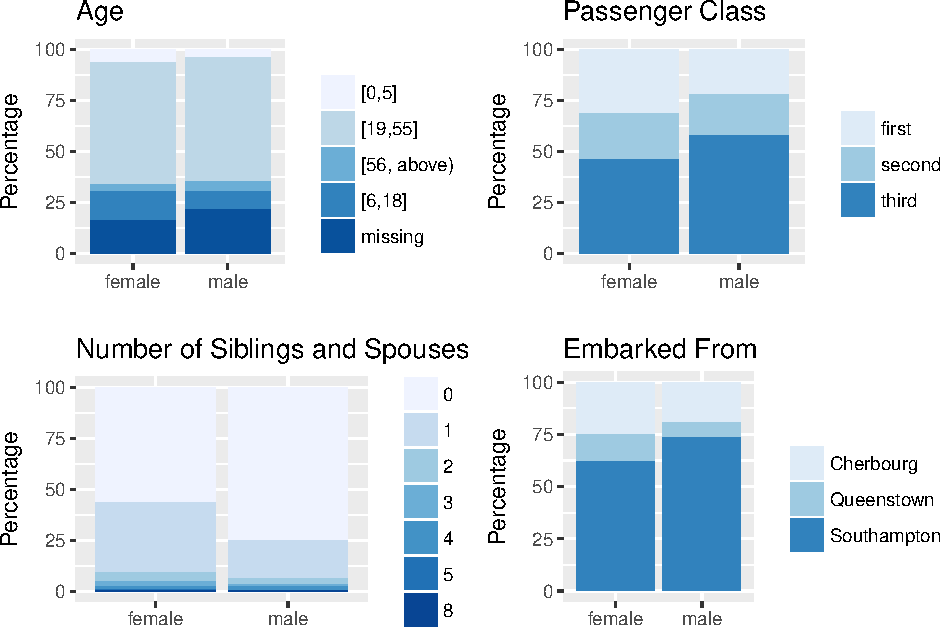
\includegraphics{report_files/figure-latex/unnamed-chunk-14-1.pdf}

It seems that there is no significant correlation between \texttt{age}
and \texttt{gender}, or \texttt{embarked\_from} and \texttt{gender}.
There is, however, a significant difference in the proportion of between
the passenger classes for each gender. The number of siblings and
spouses also seems to be correlated with gender. Because of this, we
considered making two models, one with \texttt{gender} and one without
\texttt{gender}.

Also, we looked at the correlation of \texttt{embarked\_from} and
\texttt{passenger\_class}; the plot is shown below:

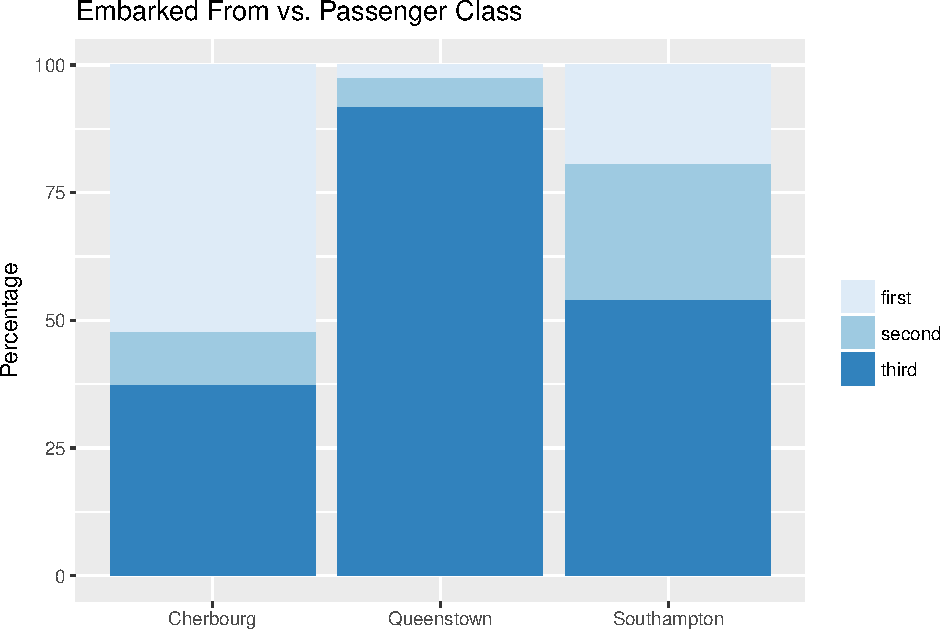
\includegraphics{report_files/figure-latex/unnamed-chunk-15-1.pdf}

As can be seen from this graph, there is a very significant correlation
between \texttt{passenger\_class} and \texttt{embarked\_from}. For
example, more than half of the passengers from Cherbourg are first class
passengers, and only a few from Queenstown are first class. This
suggests that we should be very careful when include both
\texttt{passenger\_class} and \texttt{embarked\_from} in the same model.

Next, we created the following models. The one without \texttt{gender}
takes \texttt{passenger\_class}, \texttt{age} and
\texttt{number\_of\_siblings\_and\_spouses} into account. We tried
several models, and despite the fact that we will get a better p-value
from Hosmer-Lemeshow goodness-of-fit test by including
\texttt{embarked\_from}, we still think it might be problematic because
of its strong association with \texttt{passenger\_class}. The summary of
the best model (without \texttt{gender}) found and the result from the
Hosmer-Lemeshow goodness-of-fit test is as shown:

\begin{verbatim}
## 
## Call:
## glm(formula = has_survived ~ passenger_class + age + number_of_siblings_and_spouses, 
##     family = binomial(link = "logit"), data = titanic)
## 
## Deviance Residuals: 
##     Min       1Q   Median       3Q      Max  
## -2.1791  -0.8806  -0.7015   0.9754   2.1284  
## 
## Coefficients:
##                                Estimate Std. Error z value Pr(>|z|)    
## (Intercept)                     2.43417    0.35008   6.953 3.57e-12 ***
## passenger_classsecond          -0.97894    0.17462  -5.606 2.07e-08 ***
## passenger_classthird           -1.78063    0.15635 -11.389  < 2e-16 ***
## age[19,55]                     -1.78069    0.32160  -5.537 3.08e-08 ***
## age[56, above)                 -2.80888    0.44150  -6.362 1.99e-10 ***
## age[6,18]                      -1.24306    0.34932  -3.558 0.000373 ***
## agemissing                     -1.93037    0.34351  -5.620 1.91e-08 ***
## number_of_siblings_and_spouses -0.15772    0.07244  -2.177 0.029468 *  
## ---
## Signif. codes:  0 '***' 0.001 '**' 0.01 '*' 0.05 '.' 0.1 ' ' 1
## 
## (Dispersion parameter for binomial family taken to be 1)
## 
##     Null deviance: 1736.2  on 1305  degrees of freedom
## Residual deviance: 1557.0  on 1298  degrees of freedom
## AIC: 1573
## 
## Number of Fisher Scoring iterations: 4
\end{verbatim}

\begin{verbatim}
## 
##  Hosmer and Lemeshow goodness of fit (GOF) test
## 
## data:  titanic$has_survived, fitted(m_best_8)
## X-squared = 9.1521, df = 6, p-value = 0.1652
\end{verbatim}

As we mentioned before, this p-value is not the best that could be
achieved, but it is still good enough given that it is greater than
0.05. The equation of this regression model is:
\[ln(\hat{\frac{p}{1-\hat{p}}})= 2.43417 -1.24306 \times age[6,18] -1.78069 \times age[19,55] -2.80888 \times age[56, above)\\ -1.93037\times agemissing -0.15772 \times number\_of\_siblings\_and\_spouses\\ -0.97894\times passenger\_classsecond -1.78063\times passenger\_classthird\]
The negative coefficients of all variables suggest that the reference
group is the group with highest survival rate. That is the group of
children (age smaller than 5) in first class without any siblings and
spouses are the most likely to survive; and the natural log of odds is
expected to be 2.43. This means that their chance of survival is
approximately 0.9190865. There are many other interesting interpretation
that can be extracted from this model. For example, it suggests that
first class passengers are expected to have a 0.98 higher natural log of
odds than second class passengers, all else held constant. Also, we can
expect a decrease of 0.16 in natural log of odds for every one more
increase in number of siblings and spouses, all else held constant.

This model seems good as it matches with our instinct that children and
first class passengers will have better chance of survival in a
shipwreck. This could be due to their proximity to the rescue site, or
perhaps, first class passengers were more likely to know how to swim
given their background. However, since \texttt{gender} is such an
important variable, we would also like to examine a model with
\texttt{gender} as one of the explanatory variables.

We made a set of models and compared them according to their meanings
and their results from Hosmer-Lemeshow goodness-of-fit test. It turns
out that all the model with \texttt{gender} variable fails the
Hosmer-Lemeshow goodness-of-fit test since they all have really really
low p-value, but arguably, we could conclude that the best model (with
\texttt{gender}) is the one that takes \texttt{gender}, \texttt{age},
\texttt{passenger\_class}, and
\texttt{number\_of\_siblings\_and\_spouses} because it contains the most
crucial information of a passenger, and its AIC value is the lowest
among all the models including \texttt{gender} as an explanatory
variable. The summary of this model is as shown below:

\begin{verbatim}
## 
## Call:
## glm(formula = has_survived ~ gender + age + number_of_siblings_and_spouses + 
##     passenger_class, family = binomial(link = "logit"), data = titanic)
## 
## Deviance Residuals: 
##     Min       1Q   Median       3Q      Max  
## -2.8653  -0.6894  -0.4535   0.6856   2.5462  
## 
## Coefficients:
##                                Estimate Std. Error z value Pr(>|z|)    
## (Intercept)                     4.46068    0.44952   9.923  < 2e-16 ***
## gendermale                     -2.61030    0.15445 -16.901  < 2e-16 ***
## age[19,55]                     -2.01284    0.38663  -5.206 1.93e-07 ***
## age[56, above)                 -3.08942    0.52946  -5.835 5.38e-09 ***
## age[6,18]                      -1.70756    0.42644  -4.004 6.22e-05 ***
## agemissing                     -2.15090    0.41233  -5.217 1.82e-07 ***
## number_of_siblings_and_spouses -0.37239    0.09176  -4.058 4.95e-05 ***
## passenger_classsecond          -1.11954    0.20723  -5.402 6.57e-08 ***
## passenger_classthird           -1.92213    0.18536 -10.369  < 2e-16 ***
## ---
## Signif. codes:  0 '***' 0.001 '**' 0.01 '*' 0.05 '.' 0.1 ' ' 1
## 
## (Dispersion parameter for binomial family taken to be 1)
## 
##     Null deviance: 1736.2  on 1305  degrees of freedom
## Residual deviance: 1204.1  on 1297  degrees of freedom
## AIC: 1222.1
## 
## Number of Fisher Scoring iterations: 5
\end{verbatim}

\begin{verbatim}
##                   y0  y1     yhat0      yhat1
## [0.00548,0.0977] 195  22 199.42682  17.573180
## (0.0977,0.111]   205  42 219.77092  27.229080
## (0.111,0.144]     26   6  27.56544   4.434556
## (0.144,0.225]    148  18 132.71261  33.287390
## (0.225,0.459]    122  63 109.91946  75.080540
## (0.459,0.628]     81  87  70.01437  97.985627
## (0.628,0.798]     21 108  32.54474  96.455263
## (0.798,0.984]     10 152  16.04564 145.954365
\end{verbatim}

\begin{verbatim}
## 
##  Hosmer and Lemeshow goodness of fit (GOF) test
## 
## data:  titanic$has_survived, fitted(m_best_12)
## X-squared = 33.874, df = 6, p-value = 7.114e-06
\end{verbatim}

As we can see from the summary, the equation of this regression model is
\[ln(\hat{\frac{p}{1-\hat{p}}})= 4.46068 -2.61030 \times gendermale -2.01284 \times age[19,55] -3.08942 \times age[56, above) \\-1.70756 \times age[6,18] -2.15090\times agemissing -0.37239 \times number\_of\_siblings\_and\_spouses\\ -1.11954\times passenger\_classsecond -1.92213\times passenger\_classthird\]
Since all the coefficients are negative, the reference group is expected
to be the group of people with highest chance of survival, similar to
the previous model. That is, little girls (age under 5) in first class
without siblings and spouses are ones with highest survival chance; and
the natural log of odds is expected to be 4.46, which means that their
chance of survival is approximately 0.9885698. Also, the coefficients
suggest how each variable affect the chance of survival. For example,
males are expected to have a 2.61 lower natural log of odds than
females, all else held constant. We can also see that having one more
siblings or spouses is associated with 0.37 decrease in natural log of
odds, all else held constant.

As for the best model between these two, we chose the latter one,
i.e.~the model with \texttt{gender} variable. We find it interesting to
look at the correlation between \texttt{gender} and
\texttt{has\_survived}.

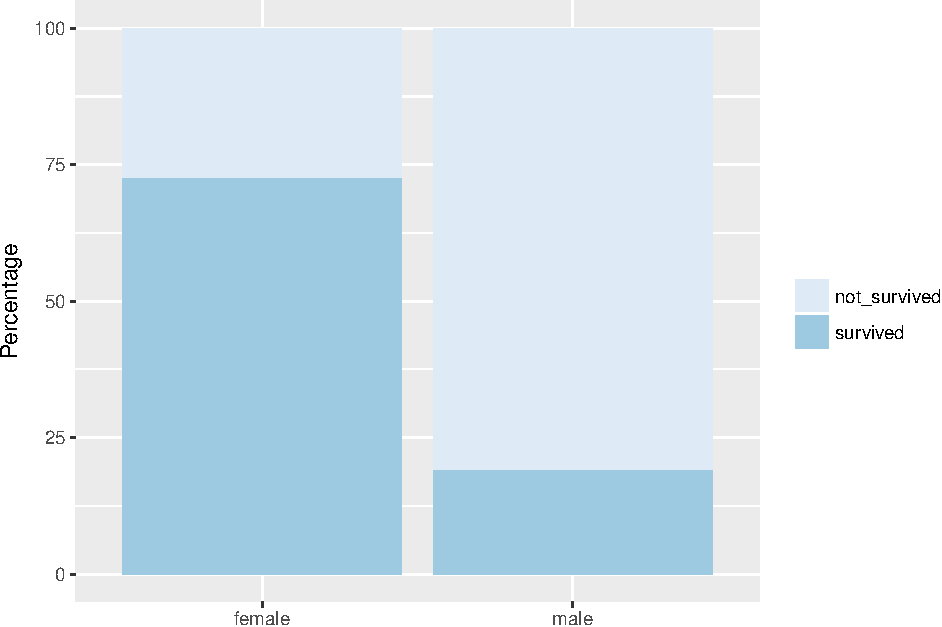
\includegraphics{report_files/figure-latex/unnamed-chunk-19-1.pdf}

From the graph, we can see that a majority of female survived while much
lower percentage of male survived, so there is indeed, a very strong
correlation between \texttt{gender} and \texttt{has\_survived}. Thus, we
think it makes more sense to have \texttt{gender} as one of the
explanatory variables in the final model, even if including it causes a
decrease in the p-value of Hosmer-Lemeshow goodness-of-fit test result.
Also, the AIC decreases significantly after we added \texttt{gender} in
the model. This suggests that including \texttt{gender} will make our
model a better fit even if we take penalty of adding new variables.
Hence, we conclude our best model as:

\[ln(\hat{\frac{p}{1-\hat{p}}})= 4.46068 -2.61030 \times gendermale -2.01284 \times age[19,55] -3.08942 \times age[56, above) \\-1.70756 \times age[6,18] -2.15090\times agemissing -0.37239 \times number\_of\_siblings\_and\_spouses\\ -1.11954\times passenger\_classsecond -1.92213\times passenger\_classthird\]

\hypertarget{conclusion}{%
\chapter{Conclusion}\label{conclusion}}

In this research, we attempted to answer the question \textbf{``How do
various demographic and socioeconomic factors affect chance of survival
in shipwreck where the ship's capacity is at least 1000 passegners and
the route is through the Atlantic Ocean in the early
20\textsuperscript{th} century?''} and we have found a not-so-surprising
result that women, children, and first class passengers have better
chance of survival. Besides, there is an interesting finding we found
that people with more siblings and spouses are less likely to survive.

As mentioned, the Hosmer-Lemeshow goodness-of-fit test p-value for the
final model is very low (7.114e-06); this suggests a lack of fit in the
model. This might also hint on the fact that generalized linear model
might not be the best approach to answer the research question, and
thus, we should try out different modelling methods. Again, as mentioned
before, AIC value only suggests if a model is relatively better than
another but does not provide an absolute scale to estimate how well a
model performs. Also, among the explanatory variables used in the model,
\texttt{age} has approximately 20\% missing data; this adds unnecessary
complexity in the model and thus could have affected the performance of
the model. Another limitation is that we only build the model but did
not really test it against real data; what we could have done is to
split the data into training and testing groups, however that is out of
the scope of the class and the project. If we can run the model against
test samples, we will have a much better sense of how the model perform.

Another the point to note is that we only have access to information of
1300/2200 passengers on the Titanic, hence our data might not have
reflected the true demographics and socioeconomic settings of passengers
on the ship. We are not so sure why there are many people missing. If
these people are majorly male labor and third-class passengers, our
findings might not been affected much. But if many of these are rich
people who tried to keep their identity hidden for example or they all
did not survived the shipwreck (so that we do not have any information
about them), then definitely our model could not generalize well.

We also consider some opportunities for further studies, which includes
splitting the data set by gender and come up with models for each part
of the data to see whether we can come up with models with better
diagnostic results for each gender. We are considering splitting the
children group (age 0-5) based on their passenger classes to see if
first class children have higher rate of survival. The only problem is
that the sample size might be too small and also there are a lot of
missing data for age.

To conclude, out of curiosity, we attempt to reimagine the night of the
disaster, putting ourselves in the shoes of those tragic passengers. As
one-score-and-two male who are properly only rich enough to get a
third-class ticket on the Titanic, we realize our inevitable fate. We
will go down with the ship, as the saying goes\ldots{}

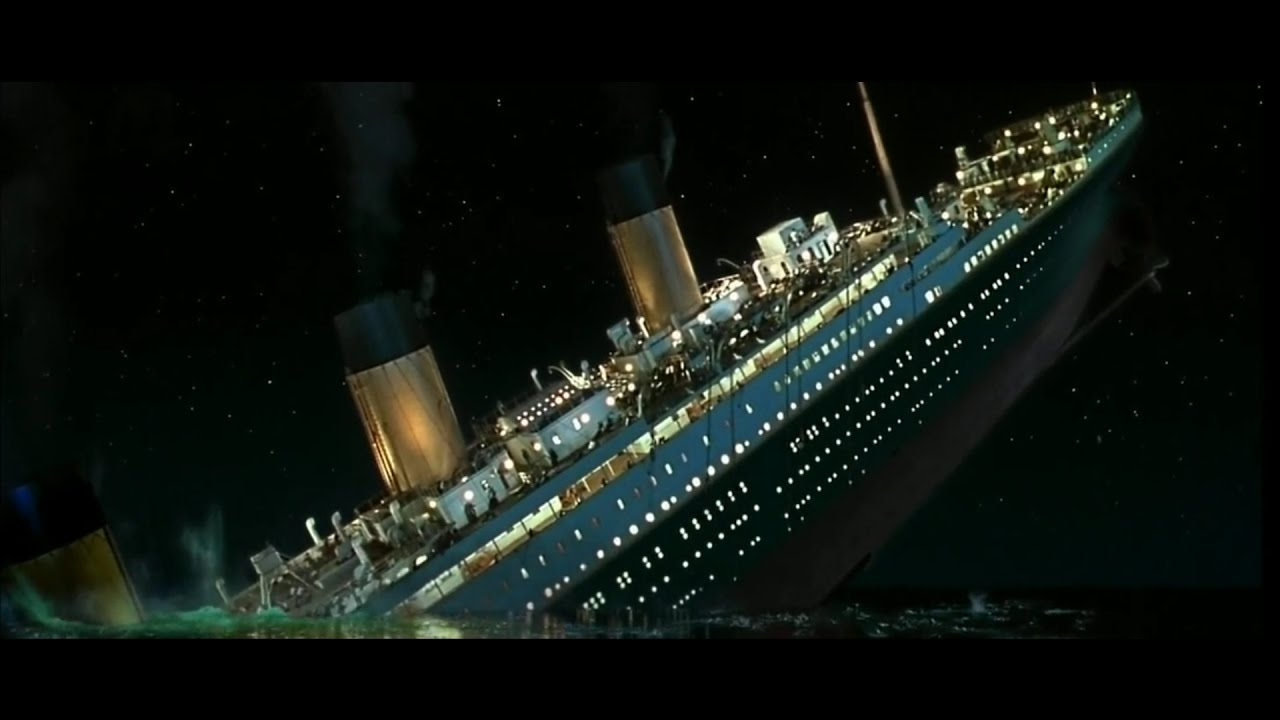
\includegraphics{assets/sinking2.jpg}

\bibliography{book.bib,packages.bib}

\end{document}
